\documentclass[12pt,a4paper]{article}
% The following LaTeX packages must be installed on your machine: amsmath, authblk, bm, booktabs, caption, dcolumn, fancyhdr, geometry, graphicx, hyperref, latexsym, natbib
\input{192.dat}
\usepackage{gensymb}
\usepackage{float}
\usepackage{siunitx}
\usepackage{amssymb}
\usepackage{float}
\usepackage{listings}
\PassOptionsToPackage{hyphens}{url}\usepackage{hyperref}
\usepackage[none]{hyphenat}
%\renewcommand{\familydefault}{\sfdefault}


\begin{document}

\setcounter{page}{1}

\section*{Exam 2}

\begin{figure}[!h]
	\centering
	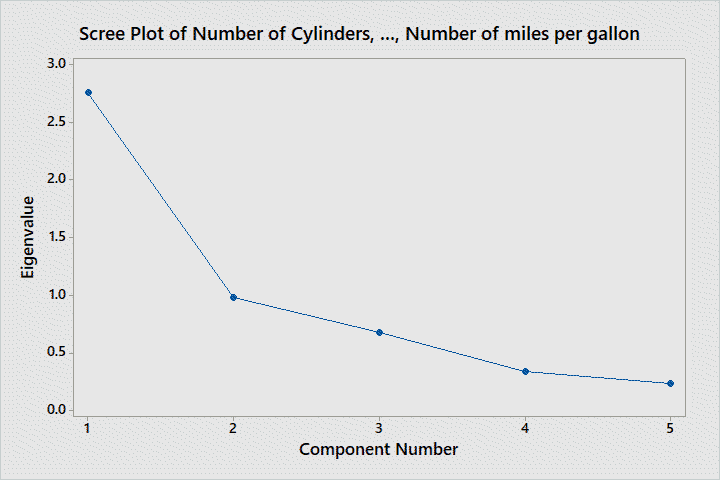
\includegraphics[width=0.7\linewidth]{pca-scree.png}
	\caption{Scree plot.}
	\label{fig:scree}
\end{figure}

\begin{figure}[!h]
	\centering
	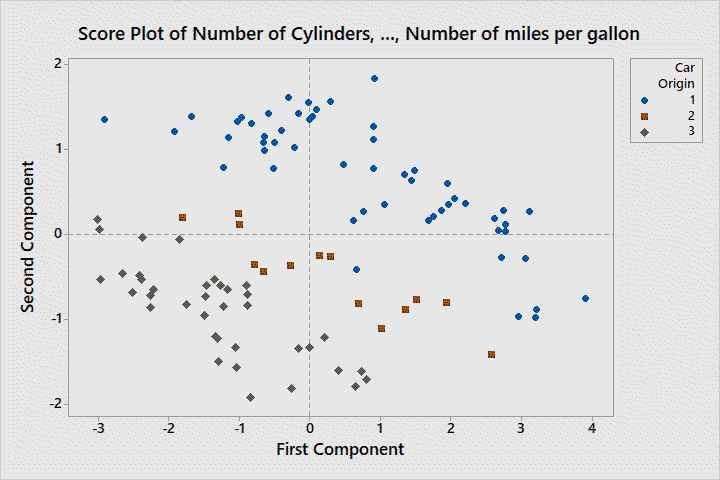
\includegraphics[width=0.7\linewidth]{pca-score.png}
	\caption{Score plot.}
	\label{fig:score}
\end{figure}

The scree plot in Figure \ref{fig:scree} shows a steep curve formed by components 1 and 2, followed by a bend and a straight line. Therefore, the components of interest are 1 and 2, which we display as a score plot in Figure \ref{fig:score}. The score plot shows clustering of the components coming from different car origins. The components appear to scale linearly with respect to the car origin, wherein car origin 1 has higher values for both component 1 and 2. This also indicates that the data is not normally distributed, but rather there are three different distributions corresponding to the car origins, as shown by the differentiation of the markers.

\end{document}